\section{Endpoint-Planning Decoupling Phenomenon}

\subsection{The CEM Compatibility Gap}

With the audit protocol established, we now define the central diagnostic. Endpoint evaluation asks whether a learned cost ranks terminal states correctly. CEM planning asks whether that cost ranks the actions sampled by the optimizer. We measure the difference with
\[
\DeltaCEM = \Rendpoint - \Rpool .
\]
Here $\Rendpoint$ is the Spearman correlation between model cost and physical task cost $C_\mathrm{real\_state}$ on a fixed endpoint artifact. $\Rpool$ uses the same costs and targets, but on the final 300-candidate pool produced by CEM. Thus $\Rendpoint$ tests global endpoint geometry, while $\Rpool$ tests the local cost landscape induced by search. A positive $\DeltaCEM$ means endpoint evaluation overstates the geometry available to the planner.

We also track $M_\mathrm{pool\_success}$, the fraction of final-pool candidates that would succeed, and $M_\mathrm{rank1}$, the success rate of the cost-selected action. Selection regret is
\[
C_\mathrm{real\_state}(a_\mathrm{rank1}) -
\min_{a\in \mathcal{P}} C_\mathrm{real\_state}(a),
\]
where $\mathcal{P}$ is the final CEM pool. These metrics separate representation quality, pool quality, and final selection.

\subsection{Cross-protocol evidence}

This subsection applies the gap metric under matched planning protocols. We evaluated a $2\times2$ grid: PushT and OGBench-Cube, crossed with full projected CEM and re-rank-only. Full projected CEM uses projected cost during elite and rank-1 selection; re-rank-only runs default CEM first, then re-ranks the final pool, separating optimization effects from final selection effects.

Table~\ref{tab:cem-gap-protocols} shows representative dimensions. Across all four protocol cells, $\Rendpoint$ increases with projection dimension while $\Rpool$ stays close to zero; at $m=64$, the PushT gaps are 0.432 and 0.394, and Cube gaps are 0.569 and 0.567. Endpoint costs that appear well-structured on fixed records become weak rankers inside final CEM pools.

\begin{table}[t]
\centering
\small
\begin{tabular}{llccccc}
\toprule
Environment & Protocol & $m$ & $\Rendpoint$ & $\Rpool$ & $\DeltaCEM$ & $M_\mathrm{rank1}$ (\%) \\
\midrule
PushT & Full projected CEM & 8 & .379 & .080 & .299 & 20.6 \\
PushT & Full projected CEM & 64 & .473 & .040 & .432 & 29.6 \\
PushT & Full projected CEM & 192 & .495 & .067 & .428 & 34.4 \\
PushT & Re-rank-only & 8 & .379 & .073 & .306 & 33.0 \\
PushT & Re-rank-only & 64 & .473 & .079 & .394 & 35.3 \\
PushT & Re-rank-only & 192 & .495 & .095 & .400 & 34.0 \\
\midrule
Cube & Full projected CEM & 8 & .477 & .001 & .476 & 52.7 \\
Cube & Full projected CEM & 64 & .575 & -.003 & .578 & 56.0 \\
Cube & Full projected CEM & 192 & .603 & .010 & .593 & 62.0 \\
Cube & Re-rank-only & 8 & .477 & .005 & .472 & 43.3 \\
Cube & Re-rank-only & 64 & .575 & .008 & .567 & 49.7 \\
Cube & Re-rank-only & 192 & .603 & .006 & .597 & 47.7 \\
\bottomrule
\end{tabular}
\caption{Endpoint and CEM-pool ranking across environments and protocols. Each row reports projection dimension $m$, endpoint Spearman correlation $\Rendpoint$ on fixed endpoint artifacts, final-pool Spearman correlation $\Rpool$ on the 300-candidate pool produced by CEM, the gap $\DeltaCEM$, and rank-1 planning success. Success values are percentages.}
\label{tab:cem-gap-protocols}
\end{table}

Figure~\ref{fig:hero} visualizes the same endpoint-pool split across projection dimensions and protocols.

\begin{figure*}[t]
\centering
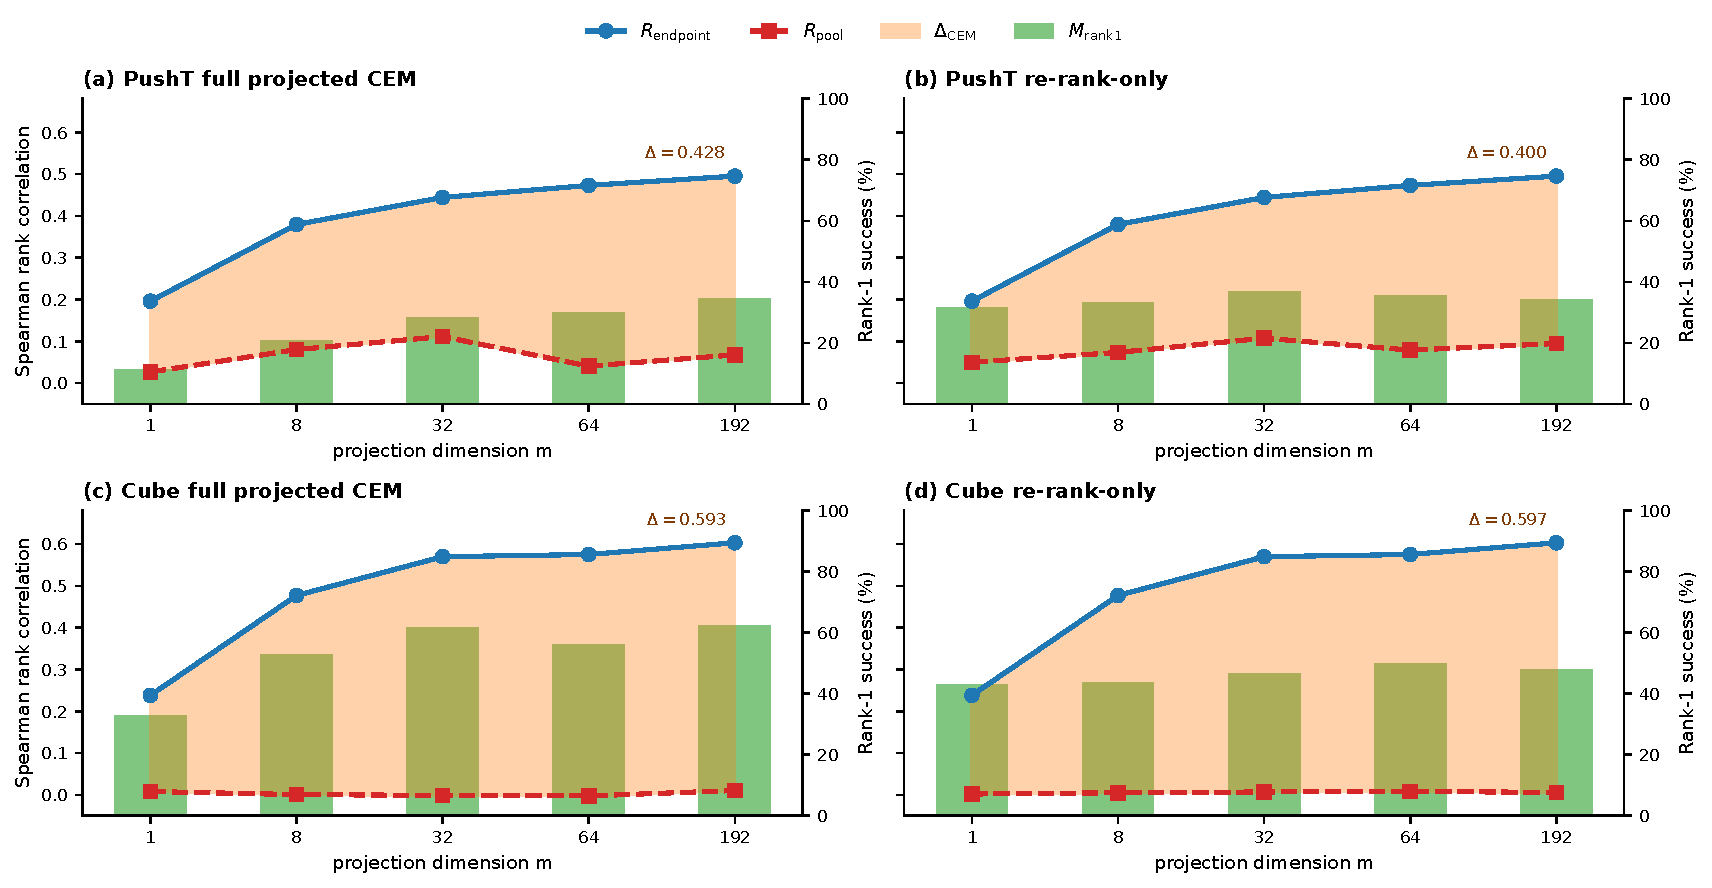
\includegraphics[width=\textwidth]{figures/fig3_enhanced.pdf}
\caption{Planning-compatible geometry diagnostics across PushT and OGBench-Cube protocols. Blue lines show endpoint Spearman rank correlation $\Rendpoint$ on fixed endpoint artifacts; red dashed lines show final-pool Spearman rank correlation $\Rpool$ on the 300 candidates retained by CEM; orange fill marks $\DeltaCEM=\Rendpoint-\Rpool$ at each projection dimension; green bars show rank-1 planning success in percent. The figure compares whether endpoint geometry transfers to the local candidate pools from which CEM selects actions.}
\label{fig:hero}
\end{figure*}

The success curves show why endpoint ranking alone is insufficient. PushT full projected CEM has a dimension elbow, from 11.1\% at $m=1$ to 34.4\% at $m=192$, while re-rank-only changes by only 2.7 percentage points. In the extended Cube full projected-CEM run, success rises from 32.7\% at $m=1$ to 61.3\% at $m=32$ and remains high at $m=64$ and $m=192$ (56.0\% and 62.0\%). Thus the original Cube inverted-U success pattern does not persist at 50-pair, three-seed scale, but the endpoint-pool ranking gap remains. Endpoint curves rise, pool curves remain low, and success can move without pool-ranking recovery.

% REVISION: addresses W3
The Cube full projected-CEM cell now uses 50 pairs and three projection seeds, compared with 100 pairs and three seeds for Cube re-rank-only. We therefore use Cube as strengthened cross-environment evidence for the endpoint-pool diagnostic, while treating detailed Cube success-curve shape as secondary.

\subsection{Five-case taxonomy}

The gap metric identifies decoupling, while $\Rendpoint$, $\Rpool$, $M_\mathrm{pool\_success}$, and $M_\mathrm{rank1}$ separate planning failure from rank-insensitive success. Table~\ref{tab:taxonomy} converts those metrics into five diagnostic cases.

\begin{table}[t]
\centering
\small
\resizebox{\textwidth}{!}{%
\begin{tabular}{llllllL{0.24\linewidth}}
\toprule
Case & $\Rendpoint$ & $\Rpool$ & $M_\mathrm{pool\_success}$ & $M_\mathrm{rank1}$ & Interpretation & Observed status \\
\midrule
A & high & high & any & high & Endpoint geometry transfers to planning & Observed in high-dimensional subset cells \\
B & high & low & high & high & Pool already good; ranking less important & Observed in Cube projections \\
C & high & low & low & low & Endpoint geometry fails as planning signal & Observed in PushT failure subsets \\
D & low & high & any & high & Local CEM geometry emerges despite poor global metric & Not observed \\
E & medium & near-zero & medium & high & Rank-insensitive success in a locally sufficient pool & Observed by the PushT ordinary stability check \\
\bottomrule
\end{tabular}}
\caption{Taxonomy for endpoint-planning relations. The cases distinguish endpoint representation quality, final-pool rank quality, success mass in the final pool, and success of the cost-selected rank-1 action.}
\label{tab:taxonomy}
\end{table}

Under strict thresholding, Case A appears in 18 subset-level cells, mainly ordinary and latent-favorable PushT cells at medium to high dimensions, but no aggregate protocol cell has Case A structure. Case B covers Cube projected protocols, Case C covers PushT invisible-quadrant failures, Case E covers rank-insensitive PushT ordinary success, and Case D is absent.

% REVISION: addresses W2
\subsection{Mechanism attribution: convergence compression versus local representation failure}

The pool-level collapse could reflect two different mechanisms. One possibility is convergence compression: CEM may contract the final pool into a physically narrow neighborhood where any endpoint cost has little residual order to recover. A second possibility is local representation failure: a privileged ranker may still order candidates inside the same pool, while the learned Euclidean cost $\Cmodel$ loses local order preservation. To separate these mechanisms, we recomputed $\Rpool$ on the same PushT default CEM pools using a privileged V1 hinge oracle cost, denoted $C_\mathrm{V1}$, and compared it with $\Rpool(\Cmodel)$.

Across the 100 PushT pairs, the learned Euclidean cost gives $\Rpool(\Cmodel)=0.084$, while the V1 oracle gives $\Rpool(C_\mathrm{V1})=0.666$. The same pattern holds in the hard subsets. In the 16 invisible-quadrant pairs, where the final pools contain little success mass ($M_\mathrm{pool\_success}=1.4\%$), $\Rpool(C_\mathrm{V1})=0.775$ while $\Rpool(\Cmodel)=0.022$. In the 21 sign-reversal pairs, $\Rpool(C_\mathrm{V1})=0.925$ while $\Rpool(\Cmodel)=-0.040$. Even in the latent-favorable subset, where the learned cost performs comparatively better, V1 remains stronger: $\Rpool(C_\mathrm{V1})=0.417$ versus $\Rpool(\Cmodel)=0.197$.

These numbers rule out pure CEM convergence compression as the dominant explanation and clearly exceed the pre-registered ``mixed'' zone. The mixed rule was designed for cases where the privileged ranker itself had only weak final-pool signal, e.g., $\Rpool(C_\mathrm{V1}) \in [0.05,0.15]$. Here $\Rpool(C_\mathrm{V1})=0.666 \gg 0.15$ while $\Rpool(\Cmodel)=0.084 \approx 0$, so the overall 100-pair result fits the local-representation-failure pattern: V1 retains substantial ranking power inside the CEM final pool, whereas the learned Euclidean cost does not. Per subset, the invisible-quadrant and sign-reversal groups show the strongest representation failure; ordinary and latent-favorable pairs retain partial learned-cost signal alongside stronger V1 signal. Figure~\ref{fig:v1_attribution} shows the same attribution at pair level.

\begin{figure}[t]
\centering
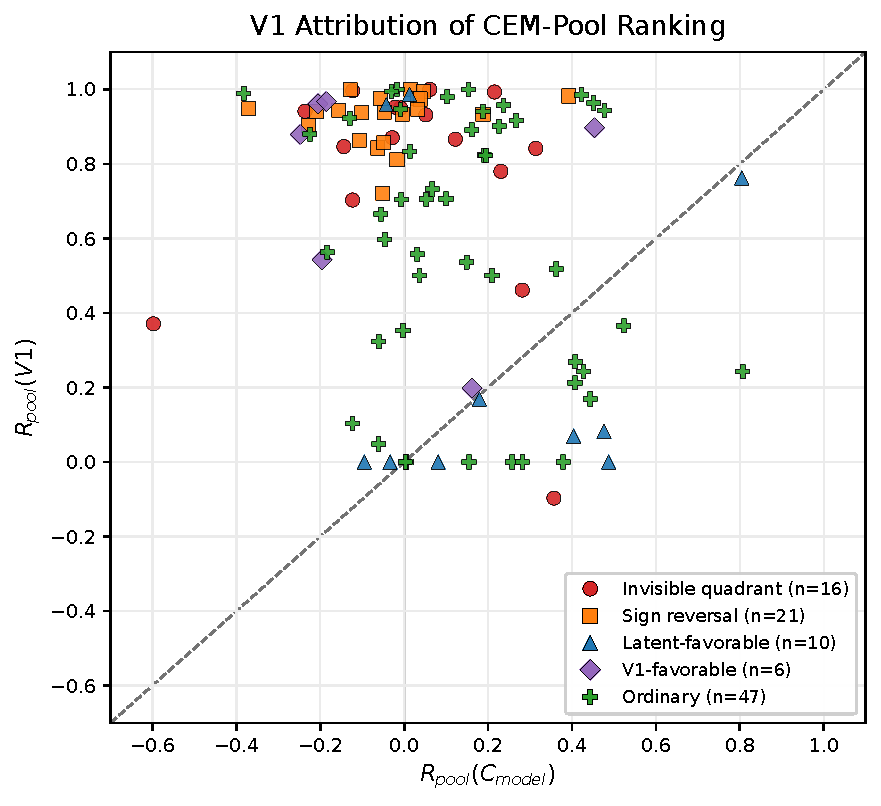
\includegraphics[width=0.72\textwidth]{figures/fig_new_a_attribution.pdf}
\caption{V1 attribution on the 100 PushT final CEM pools. Each point is one pair, with $x=\Rpool(\Cmodel)$ and $y=\Rpool(C_\mathrm{V1})$; undefined V1 Spearman values from constant oracle costs are plotted with the effective value 0. The diagonal marks equal learned and privileged rank signal. Most points lie above the diagonal, especially invisible-quadrant and sign-reversal pairs, supporting local representation failure rather than pure CEM convergence compression. Overlapping anchor definitions are assigned to a single primary subset in the legend to keep one point per pair.}
\label{fig:v1_attribution}
\end{figure}

\subsection{Per-subset structure in PushT}

\begin{figure}[t]
\centering
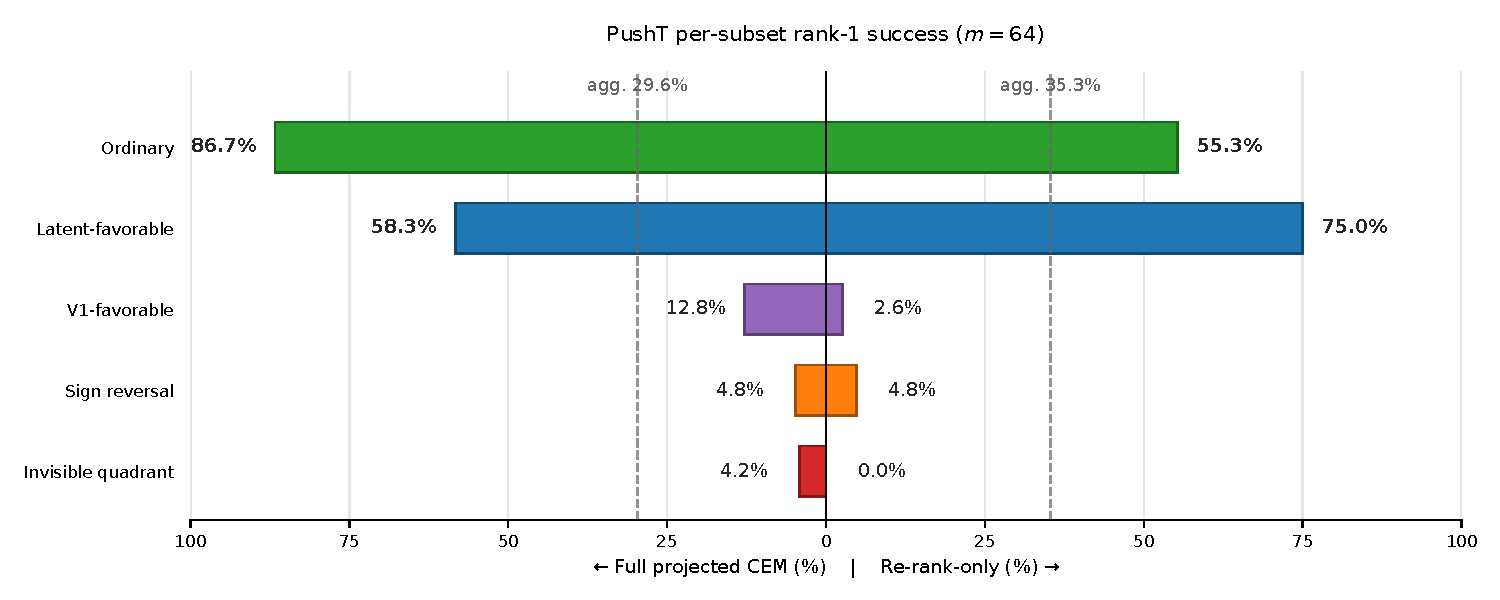
\includegraphics[width=\textwidth]{figures/fig4_butterfly.pdf}
\caption{Per-subset rank-1 planning success ($M_\mathrm{rank1}$) at projection dimension $m=64$ under two PushT protocols, shown as a butterfly chart. Leftward bars show full projected CEM and rightward bars show re-rank-only, with colors denoting subset membership. Dashed vertical lines mark aggregate success on each side. Ordinary pairs reach 86.7\% under full projected CEM, while latent-favorable pairs rise to 75.0\% under re-rank-only; the aggregate masks sharply different subset behavior under both protocols.}
\label{fig:per_subset}
\end{figure}

Figure~\ref{fig:per_subset} shows why aggregate PushT rows are insufficient: invisible-quadrant pairs lack success mass, ordinary pairs can succeed despite weak pool ranking, latent-favorable pairs produce strict Case A cells, and V1-favorable pairs expose where simulator-derived hinge cost helps more than learned latent cost.
